% 04-trien-khai.tex — Chương 4: Triển khai thực nghiệm
\chapter{Triển khai thực nghiệm}
\label{ch:trienkhai}

Chương này trình bày việc triển khai hệ thống theo kiến trúc đã đề xuất ở chương
\ref{ch:kientruc}. Mục \ref{sec:moitruong} mô tả môi trường và công cụ; mục
\ref{sec:dulieu} mô tả dữ liệu; mục \ref{sec:cai-dat-rag} trình bày cấu hình \rag; mục
\ref{sec:cai-dat-ft} trình bày thiết kế \ft; mục \ref{sec:cai-dat-agent} mô tả triển khai
multi-agent; mục \ref{sec:observability} trình bày triển khai hệ thống quan sát qua OTel
Gateway; mục \ref{sec:k8s-deploy} trình bày triển khai hệ thống lên Kubernetes; và mục
\ref{sec:khokhan} tổng kết khó khăn cùng giải pháp.

\section{Môi trường và công cụ}
\label{sec:moitruong}

Hệ thống được triển khai theo mô hình microservice trên nền Kubernetes, đóng gói bằng
Docker. Bảng \ref{tab:congcu} liệt kê các công cụ chính.

\begin{table}[htbp]
\centering
\caption{Các công cụ và thành phần chính của hệ thống.}
\label{tab:congcu}
\small
\begin{tabular}{@{}p{3.6cm}p{10.8cm}@{}}
\toprule
\textbf{Thành phần} & \textbf{Vai trò} \\
\midrule
vLLM & Phục vụ inference LLM, embedding, reranker và OCR với FP8 \\
Qdrant & Vector database, lưu dense vector và sparse \\
Kubernetes & Điều phối container, mở rộng và ổn định dịch vụ \\
Docker Compose & Triển khai cục bộ phục vụ phát triển và thử nghiệm \\
MLflow & Quản lý phiên bản prompt và gateway \\
Langfuse & Thu thập và trực quan hóa inference trace \\
OpenTelemetry & Chuẩn thu thập trace, metric, log \\
Airflow & Lập lịch thu thập và cập nhật dữ liệu định kỳ \\
PostgreSQL & Lưu trữ dữ liệu nghiệp vụ (bưu cục, tracking) \\
\bottomrule
\end{tabular}
\end{table}

\begin{figure}[htbp]
\centering
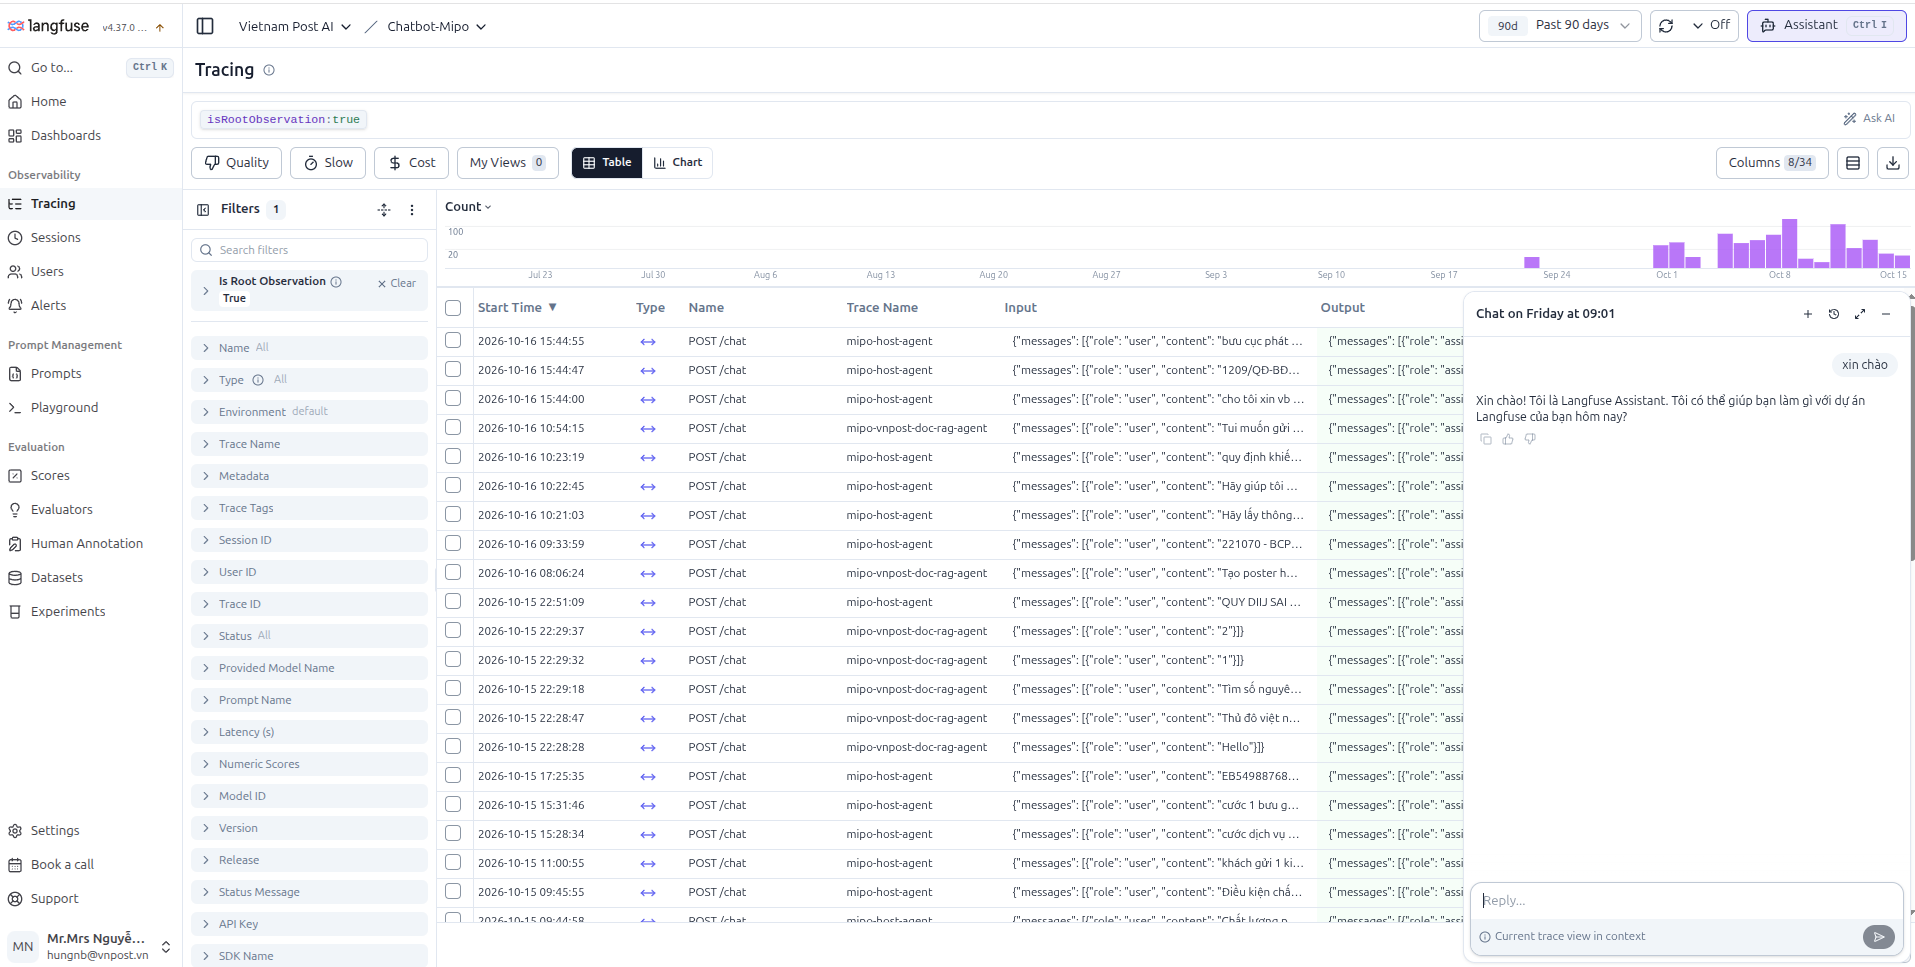
\includegraphics[width=\textwidth]{figures/hinh-4-1-langfuse-assistant.png}
\caption{Giao diện Langfuse và trợ lý AI tích hợp, dùng để quan sát và phân tích phiên hội thoại.}
\label{fig:langfuse-assistant}
\end{figure}

\section{Dữ liệu}
\label{sec:dulieu}

\subsection{Các kho tài liệu}

Đề tài sử dụng ba kho tài liệu đại diện cho các miền nghiệp vụ khác nhau, tóm tắt ở bảng
\ref{tab:corpus}.

\begin{table}[htbp]
\centering
\caption{Thống kê các kho tài liệu sử dụng trong thực nghiệm.}
\label{tab:corpus}
\small
\begin{tabular}{@{}p{4.4cm}p{2.6cm}p{6.4cm}@{}}
\toprule
\textbf{Kho tài liệu} & \textbf{Số tài liệu} & \textbf{Nội dung tiêu biểu} \\
\midrule
Văn thư nội bộ & 17 & Quyết định, công văn, quy trình nghiệp vụ \\
Sản phẩm -- dịch vụ & 119 & Biểu phí, quy định hàng hóa, bồi thường, thời gian toàn trình \\
Chuyển phát nhanh EMS & $\approx 30$ & Biểu phí EMS, quy định hàng hóa đặc biệt, bồi thường \\
\bottomrule
\end{tabular}
\end{table}

Kho tài liệu sản phẩm -- dịch vụ gồm 114 tệp văn bản, 3 tệp PDF và 2 tệp docx; sau khi
chuẩn hóa, mỗi tài liệu được sinh thêm một tệp Markdown và gắn metadata (tiêu đề, số hiệu,
ngày, tóm tắt). Kho văn thư gồm các quyết định và công văn về cước phí, thời gian toàn
trình, hàng hóa cấm gửi và chính sách bồi thường.

\subsection{Bộ mẫu đánh giá retrieval}

Đánh giá retrieval sử dụng một bộ mẫu nhỏ (6 câu hỏi) với đáp án tham chiếu, dùng để kiểm
tra chi tiết theo từng nhánh (BM25, dense), tập ứng viên sau khi hợp và bước rerank.

\subsection{Tiền xử lý}

Quy trình tiền xử lý gồm: OCR cho bản scan; chuyển đổi sang Markdown; trích xuất metadata;
structure-aware chunking; và sinh file băm (hash) để theo dõi thay đổi tài liệu. Đối
với tiếng Việt, cấu hình sparse retrieval được điều chỉnh: tắt stemming và loại bỏ danh sách
từ dừng, vì stemming tiếng Việt kém hiệu quả với thuật ngữ chuyên ngành và số hiệu văn bản.

\section{Cài đặt RAG}
\label{sec:cai-dat-rag}

\subsection{Chunking và embedding}

Văn bản được chia thành các chunk với độ dài tối đa khoảng 1000 ký tự và độ chồng lấn bảo
toàn ngữ cảnh. Bộ chunking ưu tiên ranh giới theo tiêu đề và giữ nguyên bảng. Mỗi chunk
được embedding bằng mô hình Qwen3-Embedding với vector 4096 chiều; song song đó, sparse vector
cho BM25 được tạo với chỉ số IDF.

\subsection{Cấu hình retrieval}

Bảng \ref{tab:rag-params} trình bày các tham số retrieval chính. Ở nhánh sản phẩm -- dịch vụ
của hệ thống multi-agent, số ứng viên BM25 là 10 và số ứng viên sau rerank là 10; ở
cấu hình mẫu (template) dùng cho đánh giá retrieval, các giá trị tương ứng là 20/20/5.

\begin{table}[htbp]
\centering
\caption{Cấu hình tham số retrieval RAG.}
\label{tab:rag-params}
\small
\begin{tabular}{@{}p{5.2cm}p{4.6cm}p{4.4cm}@{}}
\toprule
\textbf{Tham số} & \textbf{Cấu hình mẫu} & \textbf{Nhánh SPDV} \\
\midrule
Số ứng viên dense ($k_1^{dense}$) & 20 & 20 \\
Số ứng viên BM25 ($k_1^{bm25}$) & 20 & 10 \\
Số chunk sau rerank ($k_2$) & 5 & 10 \\
Ngưỡng điểm rerank & 0,0 & 0,0 \\
Số chiều embedding & 4096 & 4096 \\
Độ dài chunk tối đa & $\approx 1000$ & $\approx 1000$ \\
\bottomrule
\end{tabular}
\end{table}

\subsection{Embedding câu hỏi và prompt}

Câu hỏi được embedding với chỉ dẫn (instruction) phù hợp cho retrieval. Prompt hệ thống của
agent \rag{} được quản lý tập trung qua MLflow Prompt Registry (ví dụ \texttt{tct-rag-agent}),
cho phép cập nhật mà không cần triển khai lại mã nguồn. Prompt quy định rõ: chỉ trả lời dựa
trên ngữ cảnh retrieval, trích nguồn, và từ chối
khi thiếu thông tin.

\section{Thiết kế fine-tuning}
\label{sec:cai-dat-ft}

Trong ba loại mô hình, pipeline cho \textbf{embedding model} đã được thí điểm triển khai và
đánh giá thật trên Qwen3-Embedding-0.6B với một bộ dữ liệu TTHC tiếng Việt; \textbf{LLM} và
\textbf{reranker} vẫn ở mức \emph{đề xuất}. Mục này trình bày dữ liệu (\ref{sec:ft-data}) và
cấu hình huấn luyện (\ref{sec:ft-config}), cách đóng gói phục vụ (\ref{sec:ft-deploy}), rồi
các đề xuất cho LLM và reranker.

\subsection{Dữ liệu thí điểm cho embedding model}
\label{sec:ft-data}

Bộ dữ liệu gồm 199 văn bản TTHC, chia thành 179 văn bản huấn luyện và 20 văn bản kiểm định
theo tỷ lệ $0{,}1$ (hạt giống ngẫu nhiên 42 để tái lập). Sau khi khử trùng lặp theo văn bản,
tập kiểm định còn 708 truy vấn duy nhất và 1.319 đoạn văn bản. Mỗi mẫu huấn luyện là bộ ba
$(\text{query},\text{positive},\text{negative})$, với tối đa $k=3$ hard negative cho mỗi truy
vấn; tập kiểm định chia theo văn bản nên không rò rỉ chunk giữa hai tập. Bảng
\ref{tab:ft-dataset} tổng hợp thống kê.

\begin{table}[htbp]
\centering
\caption{Thống kê bộ dữ liệu thí điểm cho embedding model.}
\label{tab:ft-dataset}
\small
\begin{tabular}{@{}lr@{}}
\toprule
\textbf{Tham số} & \textbf{Giá trị} \\
\midrule
Văn bản (train / val) & 179 / 20 \\
Tỷ lệ kiểm định (theo văn bản) & 0{,}1 \\
Truy vấn (train / val) & 6.606 / 717 \\
Bộ ba (train / val) & 18.569 / 2.112 \\
Truy vấn val duy nhất & 708 \\
Đoạn văn bản val duy nhất & 1.319 \\
Số negative tối đa mỗi truy vấn & 3 \\
Negative bị loại khi làm sạch & 1.491 \\
Bộ ba bị loại (vượt hạn mức) & 990 \\
Hạt giống & 42 \\
\bottomrule
\end{tabular}
\end{table}

\subsection{Cấu hình huấn luyện và đánh giá}
\label{sec:ft-config}

Bảng \ref{tab:ft-emb-config} liệt kê cấu hình huấn luyện. Mô hình được huấn luyện trên một
GPU Tesla T4 trong 202,5 phút, bộ nhớ đỉnh được cấp phát 7,59 GB (52,1\% dung lượng GPU).
Đánh giá dùng \texttt{InformationRetrievalEvaluator} của \texttt{sentence-transformers}, với
truy vấn và kho văn bản được khử trùng lặp theo văn bản (mỗi chuỗi chỉ xuất hiện một lần, một
truy vấn có thể có nhiều positive) để tránh hiện tượng ``trần điểm giả'' khi văn bản trùng lặp
xuất hiện nhiều lần trong kho.

\begin{table}[htbp]
\centering
\caption{Cấu hình huấn luyện và đánh giá embedding model (thí điểm).}
\label{tab:ft-emb-config}
\small
\begin{tabular}{@{}p{6.4cm}p{8cm}@{}}
\toprule
\textbf{Tham số} & \textbf{Giá trị} \\
\midrule
Mô hình nền & \texttt{unsloth/Qwen3-Embedding-0.6B} \\
Phương pháp & LoRA, $r=32$, $\alpha=32$, 7 ma trận chiếu \\
Độ dài chuỗi tối đa & 1.024 token \\
Hàm mất mát & MultipleNegativesRankingLoss ($\tau^{-1}=20$) \\
Bộ lấy mẫu batch & \texttt{NO\_DUPLICATES} \\
Số epoch & 2 \\
Batch hiệu dụng & 256 (64 $\times$ 4 bước tích luỹ) \\
Tốc độ học / scheduler & $3\times10^{-5}$ / cosine, warmup 0{,}05 \\
Độ chính xác & fp16 \\
Đánh giá / checkpoint & mỗi 20 bước \\
Chỉ số chọn mô hình tốt nhất & NDCG@10 trên tập kiểm định \\
Pooling / chuẩn hoá & last-token / L2 \\
\bottomrule
\end{tabular}
\end{table}

\subsection{Đóng gói và phục vụ}
\label{sec:ft-deploy}

Adapter LoRA của checkpoint tốt nhất được gộp vào mô hình nền ở độ chính xác fp32 rồi lưu
fp16. Mô hình gộp được chuyển sang định dạng GGUF (F16) bằng \texttt{convert\_hf\_to\_gguf.py}
và lượng tử hoá về Q8\_0 bằng \texttt{llama-quantize} của \texttt{llama.cpp}~\cite{llamacpp2024};
cấu hình pooling (last-token) và chuẩn hoá L2 được giữ khớp với lúc huấn luyện. Mô hình GGUF
được phục vụ qua \texttt{llama-server} ở chế độ embedding với \texttt{-ngl 99} (đẩy toàn bộ
layer lên GPU) và \texttt{-c 2048}, cung cấp API tương thích OpenAI tại \texttt{/v1/embeddings}.
Vì mô hình không tự thêm tiền tố instruction, phía client phải thêm chuỗi tiền tố cho truy vấn
(tài liệu giữ nguyên văn bản thô).

\subsection{Đề xuất cho LLM và reranker}

Với LLM và reranker, đây vẫn là phần \emph{thiết kế đề xuất}. Bảng \ref{tab:lora} trình bày
cấu hình LoRA/QLoRA cho LLM và bảng \ref{tab:rerank-ft} cho reranker.

\begin{table}[htbp]
\centering
\caption{Cấu hình LoRA/QLoRA đề xuất cho fine-tuning LLM.}
\label{tab:lora}
\small
\begin{tabular}{@{}p{6.4cm}p{8cm}@{}}
\toprule
\textbf{Tham số} & \textbf{Giá trị đề xuất} \\
\midrule
Phương pháp & LoRA / QLoRA (4-bit NF4) \\
Hạng $r$ & 16 \\
Hệ số $\alpha$ & 32 \\
Dropout & 0,05 \\
Module áp dụng & q, k, v, o, gate, up, down \\
Tốc độ học & $1\times10^{-4}$ đến $2\times10^{-4}$ \\
Số epoch & 2--3 \\
Độ dài ngữ cảnh & 4096 token \\
Chiến lược & SFT, có thể bổ sung DPO \\
\bottomrule
\end{tabular}
\end{table}

\begin{table}[htbp]
\centering
\caption{Cấu hình fine-tuning reranker đề xuất.}
\label{tab:rerank-ft}
\small
\begin{tabular}{@{}p{6.4cm}p{8cm}@{}}
\toprule
\textbf{Tham số} & \textbf{Giá trị đề xuất} \\
\midrule
Mô hình nền & Qwen3-Reranker (cross-encoder) \\
Đầu vào & Cặp (truy vấn, chunk) \\
Nhãn & Liên quan / không liên quan theo đáp án tham chiếu \\
Hàm mất mát & Cross-entropy (phân loại) hoặc margin/ranking loss \\
Mẫu âm & Hard negatives từ top-$k$ sai \\
Hạng $r$ (nếu dùng LoRA) & 16 \\
Tốc độ học & $1\times10^{-5}$ đến $2\times10^{-5}$ \\
Số epoch & 2--4 \\
Đánh giá & Recall@5, MRR, nDCG (trước/sau) \\
\bottomrule
\end{tabular}
\end{table}

Quy trình chung cho phần đề xuất: làm sạch dữ liệu $\rightarrow$ định dạng theo loại mô hình
$\rightarrow$ chia tập theo câu hỏi $\rightarrow$ huấn luyện $\rightarrow$ đánh giá trên tập
kiểm định $\rightarrow$ đóng gói để phục vụ. Lưu ý riêng cho embedding: sau khi thay mô hình
phải \emph{re-embed toàn bộ corpus} và dựng lại chỉ mục Qdrant trước khi đo lại Recall@$k$.

\section{Triển khai multi-agent}
\label{sec:cai-dat-agent}

\subsection{Agent điều phối}

Agent điều phối (host) tiếp nhận yêu cầu, duy trì ngữ cảnh hội thoại và quyết định định
tuyến. Prompt của host quy định danh sách agent được phép gọi, tiêu chí định tuyến và cơ
chế hợp nhất kết quả. Host cũng hỗ trợ tạo ticket khi cần chuyển sang hỗ trợ thủ công, với
phân loại ticket theo nhóm nghiệp vụ (tư vấn, hỗ trợ ứng dụng, cước phí, đối soát thanh
toán, hỗ trợ kỹ thuật).

\subsection{Các agent chuyên biệt và công cụ}

Các agent chuyên biệt giao tiếp qua A2A và truy cập công cụ qua MCP. Ví dụ, agent tra cứu
bưu gửi cung cấp công cụ tra cứu theo SOAP và theo API nội bộ, cùng công cụ phân tích điểm
nghẽn (bottleneck). Agent tra cứu bưu cục truy vấn cơ sở dữ liệu PostgreSQL có tìm kiếm mờ
(fuzzy search) để xử lý sai chính tả. Agent \rag{} sản phẩm -- dịch vụ dùng Qdrant và
reranker như mô tả.

\subsection{Quy tắc định tuyến}

Với miền EMS, hệ thống sử dụng một bộ khoảng 26 quy tắc chuyển agent, được nhóm theo các
chủ đề: yêu cầu trực tiếp, khiếu nại/bồi thường, phản hồi, tác vụ vận hành, nghiệp vụ/hợp
đồng, khách hàng VIP, an ninh/pháp lý, độ tin cậy thấp và chuyển cấp. Các quy tắc được lưu
dưới dạng JSON có thể đọc bằng máy, bao gồm thông tin cần thu thập và chính sách theo giờ
hành chính, giúp việc định tuyến nhất quán và dễ bảo trì.

\begin{figure}[htbp]
\centering
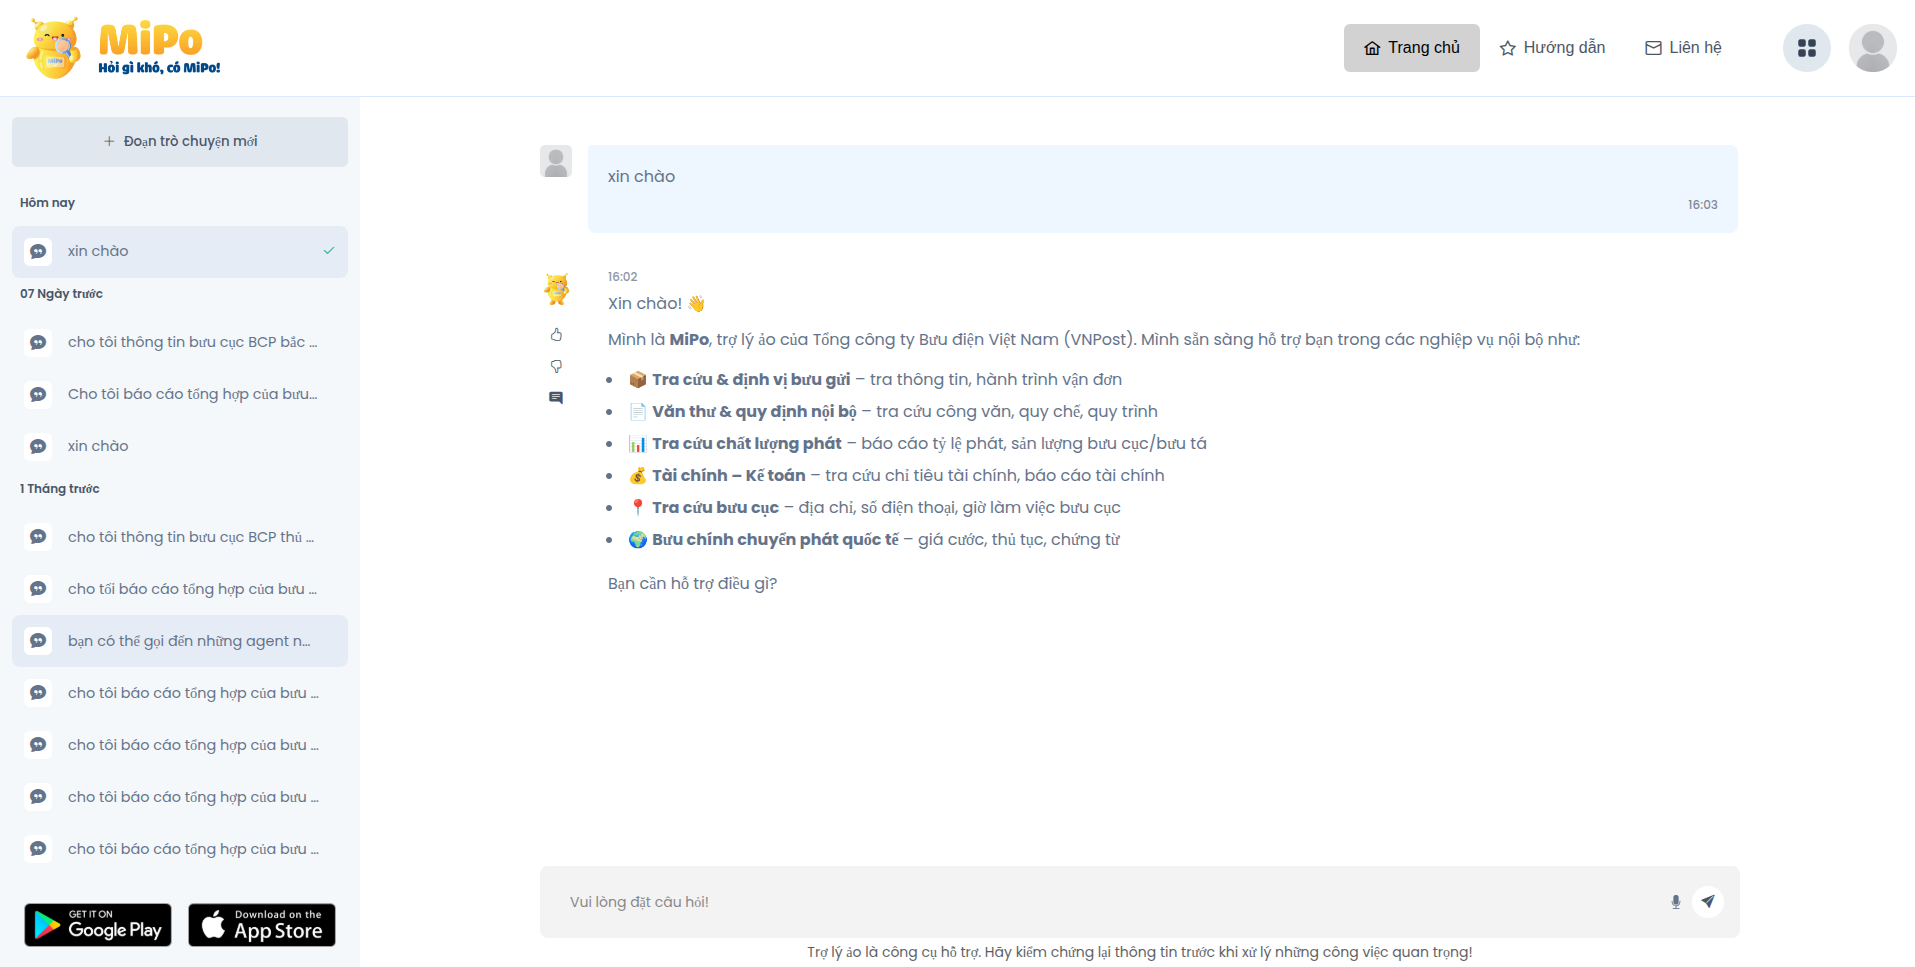
\includegraphics[width=\textwidth]{figures/hinh-4-2-chatbot-mipo.png}
\caption{Giao diện trợ lý ảo MiPo: khung hội thoại, danh sách phiên và các nhóm nghiệp vụ được hỗ trợ.}
\label{fig:chatbot-mipo}
\end{figure}

\section{Quan sát với OTel Gateway}
\label{sec:observability}

\subsection{Cấu hình OTel Gateway}

OTel Gateway được cài đặt bằng image \texttt{otel/\allowbreak opentelemetry-collector-contrib} với một
tệp cấu hình gồm ba phần: \emph{receivers}, \emph{processors} và \emph{exporters}. Receiver
\texttt{otlp} nhận vết qua gRPC ở cổng 4317 và HTTP ở cổng 4318; processor \texttt{batch}
gom các vết trước khi gửi. Pipeline \texttt{traces/langfuse} đi qua processor
\texttt{transform/langfuse} để ánh xạ attribute trung lập sang data model của Langfuse,
rồi export bằng \texttt{otlphttp/langfuse} tới endpoint ingest của Langfuse.

Exporter \texttt{otlphttp} tự POST tới \texttt{\{endpoint\}/v1/traces} với header xác thực
Basic, kèm \texttt{sending\_queue} (kích thước 1000) và \texttt{retry\_on\_failure} (chu kỳ
thử lại tăng dần từ 5 giây tới 30 giây, thời hạn 5 phút) nhằm không mất vết khi backend
chậm. Các pipeline tương tự được tạo cho \texttt{metrics} và \texttt{logs}.

\subsection{Attribute agent phát}

Mỗi agent phát attribute theo chuẩn OpenTelemetry semantic conventions, ở dạng trung lập
mọi backend. Bảng \ref{tab:otel-attr} liệt kê các attribute chính.

\begin{table}[htbp]
\centering
\caption{Attribute chính mà agent phát theo chuẩn OpenTelemetry.}
\label{tab:otel-attr}
\small
\begin{tabular}{@{}p{6.2cm}p{8.2cm}@{}}
\toprule
\textbf{Attribute} & \textbf{Ý nghĩa} \\
\midrule
\texttt{OTEL\_SERVICE\_NAME} & Tên service hiện trên trace \\
\texttt{gen\_ai.operation.name} & Loại thao tác: \texttt{chat}, \texttt{invoke\_agent}, \texttt{execute\_tool} \\
\texttt{gen\_ai.request.model} + \texttt{gen\_ai.request.*} & Mô hình và tham số sampling \\
\texttt{gen\_ai.usage.input/output/total\_tokens} & Lượng token sử dụng \\
\texttt{gen\_ai.input.messages} / \texttt{gen\_ai.output.messages} & Nội dung messages chuẩn OpenAI \\
\texttt{gen\_ai.tool.call.arguments} / \texttt{.result} & Đầu vào/đầu ra của tool \\
\texttt{gen\_ai.response.first\_token\_time} & Thời điểm sinh token đầu tiên (TTFT) \\
\texttt{session.id} / \texttt{user.id} & Định danh phiên và người dùng \\
\texttt{meta.<key>} & Metadata của request (dùng làm bộ lọc) \\
\bottomrule
\end{tabular}
\end{table}

\subsection{Ánh xạ sang Langfuse ở collector}

Phép ánh xạ được khai báo ở processor \texttt{transform/langfuse} của collector, gồm:
\texttt{service.name} làm tên trace; \texttt{meta.<key>} chuyển thành
\texttt{langfuse.trace.metadata.<key>} để lọc trong UI; loại observation suy từ
\texttt{gen\_ai.operation.name}; input/output của từng observation copy từ các attribute
tương ứng; và TTFT ánh xạ thành thời điểm bắt đầu sinh token. Langfuse tự nhận diện các
attribute chuẩn như \texttt{session.id}, \texttt{user.id}, \texttt{gen\_ai.usage.*} và
\texttt{gen\_ai.request.*} mà không cần ánh xạ thủ công.

Vì phép ánh xạ nằm ở collector, việc thêm hoặc đổi backend chỉ cần sửa tệp cấu hình
collector và khởi động lại collector -- không cần sửa code agent và không cần restart agent.
Đây là điểm chính giúp kiến trúc quan sát bền vững khi hệ thống mở rộng.

\subsection{Quy trình sử dụng}

Vết được xem trên Langfuse UI ở các tab Traces, Sessions và Agent Graph. Thông tin phiên và
người dùng được truyền qua OTel Baggage trong carrier \texttt{otel\_context} gửi kèm theo A2A/MCP;
phía nhận, baggage processor copy hai entry này lên mọi span, kể cả span sinh ra ở process
khác. Nhờ đó, một hội thoại nhiều lượt đi qua nhiều agent vẫn gom thành một session.

\begin{figure}[htbp]
\centering
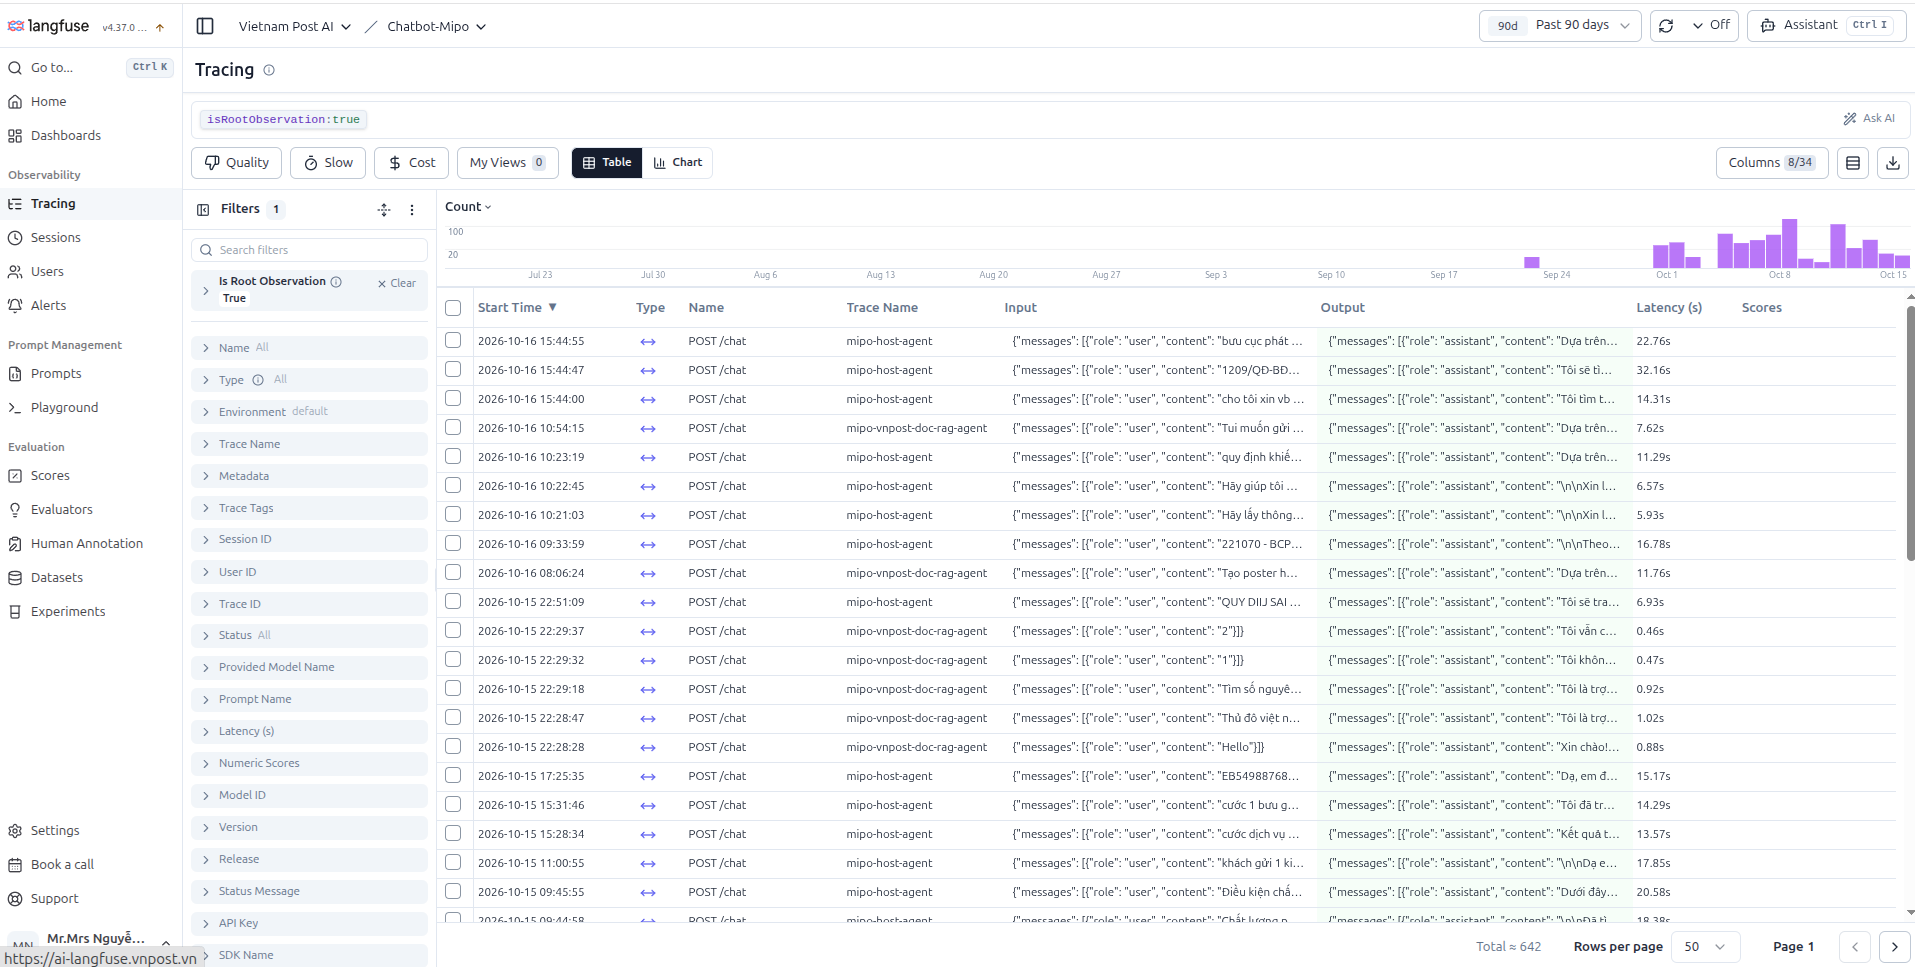
\includegraphics[width=\textwidth]{figures/hinh-4-3-langfuse-traces.png}
\caption{Danh sách trace trên Langfuse (lọc \texttt{isRootObservation=true}): mỗi dòng là một
lượt \texttt{/chat}, kèm agent xử lý và độ trễ.}
\label{fig:langfuse-traces}
\end{figure}

\begin{figure}[htbp]
\centering
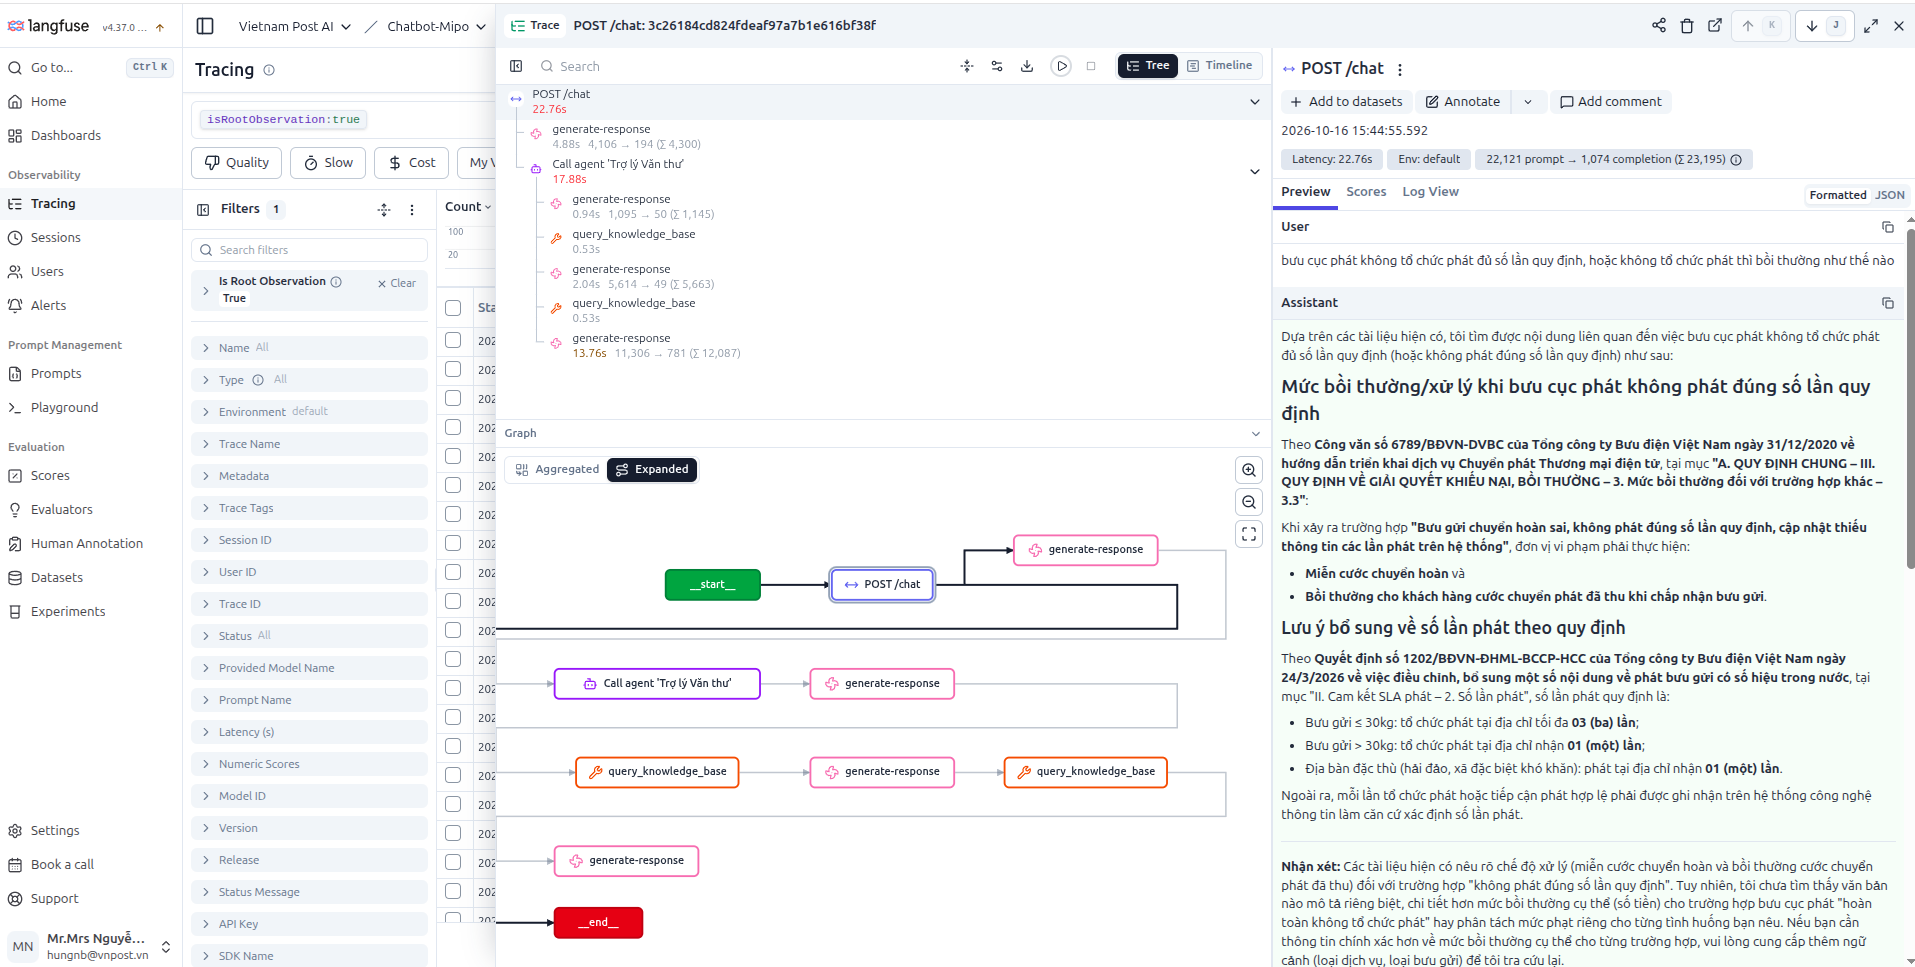
\includegraphics[width=\textwidth]{figures/hinh-4-4-langfuse-trace-detail.png}
\caption{Chi tiết một trace: các bước \texttt{generate-response}, \texttt{query\_knowledge\_base}
và lời gọi agent, kèm nội dung hội thoại và trích dẫn ở panel phải.}
\label{fig:langfuse-trace-detail}
\end{figure}

\begin{ghichu}
Quy trình đánh giá (eval) chủ động tắt OpenTelemetry, để vết của quá trình đánh giá không
lẫn vào backend quan sát và không làm nhiễu số liệu vận hành.
\end{ghichu}

Prompt được quản lý tập trung qua MLflow Prompt Registry. Mỗi agent tham chiếu một prompt
theo tên và nhãn (ví dụ \texttt{@production}), nhờ đó có thể cập nhật prompt cho tất cả
agent mà không cần sửa mã hay triển khai lại. Cơ chế này tách cấu hình khỏi logic và hỗ
trợ kiểm soát thay đổi.

\section{Triển khai hệ thống lên Kubernetes}
\label{sec:k8s-deploy}

\subsection{Tổ chức manifests}

Mỗi dịch vụ được tổ chức thành một thư mục manifests riêng gồm các nhóm tệp: \texttt{workloads}
(Deployment), \texttt{configs} (ConfigMap), \texttt{secrets} (Secret), \texttt{networks}
(Service, Ingress) và \texttt{images}. Cách tổ chức này giúp dễ quản lý, dễ tạo bản mới và
tái sử dụng cấu hình giữa các dịch vụ. Bảng \ref{tab:k8s-services} liệt kê nhóm dịch vụ
chính được triển khai.

\begin{table}[htbp]
\centering
\caption{Nhóm dịch vụ triển khai trên Kubernetes.}
\label{tab:k8s-services}
\small
\begin{tabular}{@{}p{5.4cm}p{9cm}@{}}
\toprule
\textbf{Nhóm} & \textbf{Thành phần} \\
\midrule
Workload mô hình (GPU) & LLM, embedding model, reranker, OCR \\
Workload agent (CPU) & host agent, agent RAG, agent tracking, agent bưu cục \\
Quan sát & Langfuse, OTel Gateway \\
Dữ liệu & Qdrant, PostgreSQL, MinIO \\
Nền tảng & Airflow, mem0, registry nội bộ \\
\bottomrule
\end{tabular}
\end{table}

\subsection{Workload GPU và init container}

Các Pod phục vụ mô hình yêu cầu \texttt{runtimeClassName: nvidia} để dùng GPU, và dùng
\texttt{nodeSelector} để neo về node có card đồ họa. \texttt{terminationGracePeriodSeconds}
đặt đủ dài để Pod dừng an toàn. Việc khởi động Pod có init container phụ trách chuẩn bị
dữ liệu:

\begin{itemize}
  \item \textbf{Workload mô hình:} init container tải trọng số từ máy chủ lưu trữ nội bộ
  (SFTP) về PVC; container chính sau đó khởi động vLLM và phục vụ mô hình.
  \item \textbf{Workload agent:} init container tải mã agent từ kho Git nội bộ về PVC;
  container chính sau đó chạy API server.
\end{itemize}

Cách này giữ image sát cơ bản, tách dữ liệu/biến động khỏi image, và cho phép cập nhật mô
hình hoặc mã agent mà không cần build lại image.

\subsection{Cấu hình, bản mật và kết nối nội bộ}

Cấu hình runtime đặt ở ConfigMap; thông tin nhạy cảm (khóa xác thực, khóa API) đặt ở
Secret; biến môi trường theo môi trường triển khai được quản lý cùng bộ manifests. Image
lấy từ registry nội bộ của Tổng công ty. Các tên miền nội bộ cần phân giải được khai báo
qua \texttt{hostAliases}. Trong giai đoạn phát triển và thử nghiệm cục bộ, hệ thống chạy
bằng Docker Compose; khi đưa vào vận hành thì chuyển lên Kubernetes, giữ nguyên cấu hình
logic của agent.

\section{Khó khăn và giải pháp}
\label{sec:khokhan}

\begin{table}[htbp]
\centering
\caption{Khó khăn gặp phải và giải pháp áp dụng.}
\label{tab:khokhan}
\small
\begin{tabular}{@{}p{5.2cm}p{9.2cm}@{}}
\toprule
\textbf{Khó khăn} & \textbf{Giải pháp} \\
\midrule
Stemming tiếng Việt kém hiệu quả & Tắt stemming, loại bỏ từ dừng trong BM25 \\
Bảng biểu bị cắt vụn khi chunking & Chunking nhận biết cấu trúc, bảo toàn bảng \\
Tài liệu scan chất lượng thấp & Tiền xử lý OCR bằng mô hình nhận dạng chuyên dụng \\
Reranker làm giảm recall top-$k$ nhỏ & Phân tích lỗi, điều chỉnh $k$ và ngưỡng \\
Chi phí GPU cho mô hình lớn & Quantization FP8, phục vụ theo lô với vLLM \\
Dữ liệu nhạy cảm & Chạy cục bộ, ẩn PII, RBAC theo vai trò \\
Prompt phân tán, khó kiểm soát & MLflow Prompt Registry tập trung \\
\bottomrule
\end{tabular}
\end{table}

\section*{Kết chương}
\addcontentsline{toc}{section}{Kết chương}
Chương này đã mô tả môi trường, dữ liệu, cấu hình \rag, thiết kế \ft, triển khai multi-agent
và hệ thống quan sát. Chương tiếp theo trình bày kết quả thực nghiệm và đánh giá.
